% !TEX TS-program = pdflatex
\documentclass[11pt]{article}
\usepackage[margin=1in]{geometry} 
\usepackage[parfill]{parskip}% Begin paragraphs with an empty line rather than an indent
\usepackage{graphicx}
%\pdfmapfile{+scanpages.map}
%SetFonts
% libertine+newtxmath
\usepackage[osf,sups]{baskervillef}
\usepackage[T1]{fontenc}
\usepackage{textcomp}
\usepackage[scaled=.85]{beramono}
\usepackage[scaled=.95]{cabin}
\usepackage{amsmath,amsthm}
\usepackage[baskerville]{newtxmath}
\usepackage{url}
%SetFonts
\usepackage{scanpages}
\title{The \textsf{Scanpages} Package}
\author{Michael Sharpe}
\date{\today}  % Activate to display a given date or no date

\begin{document}
\maketitle
\section{Briefly}
This package is intended for production of documents based on scanned material in any format acceptable to \textsf{pdflatex} as a graphic inclusion---eg, {\tt pdf}, {\tt png}, {\tt jpg}, though {\tt pdf} works best with this package. For me, the format has been useful when trying to archive pre-\TeX\ documents without converting them to \LaTeX\ source documents but inputting the scanned pages one by one and adding indexing, hyperlinks, a table of contents (You'll have to do this using \verb|\addcontentsline{toc}...|, and if using \textsf{hyperref}, you may need to add \verb|\phantomsection| immediately before \verb|\addcontentsline|), footnotes, marginal notes and the like. What makes scanned documents bothersome is the irregularities introduced by the scanning process. Pages are sometimes skewed and often offset horizontally and/or  vertically from one another, and extraneous marks will likely appear, so each page may need adjustments. The methods of this package are of two types. First, the package {\tt scanpages.sty} contains macros to make it more convenient to perform those adjustments and add adornments. Second, some kind of script is very useful for making the relevant part of the {\tt tex} source, if you are handling more than a few pages of scanned material. For this, there are two almost equivalent scripts included to automate this process as much as possible, one written in \textsf{python}, the other in \textsf{AppleScript.} (The letter may be installed in \TeX Shop's macro menu for completely self-contained usage.)
\section{The \LaTeX\ package}
Starting with a scanned document, you need to measure four dimensions to specify the region you wish to import, and decide on a magnification factor to apply. The region to import from the scan should ideally be a bit larger (10{\tt pt} is a good starting value) than the area typically containing all the data, and perhaps excluding original page numbers. (The part of the scanned page lying outside the region is cropped.) The four critical dimensions are:
\begin{itemize}
\item
The $x$ and $y$ coordinates {\tt llx, lly} of the lower left corner of the image region (the part you want to  import) relative to the lower left corner of the scanned page;
\item the width {\tt w} of the image region;
\item the height {\tt h} of the image region. 
\end{itemize}
The package is called using these items as options to the package.
\begin{verbatim}
\usepackage[scale=.9,llx=8cm,lly=12cm,w=3.5in,h=3.5in]{scanpages}
\end{verbatim}
It is not an error to omit one or more of these values, as default values will be substituted:
\begin{itemize}
\item
{\tt llx} and {\tt lly} default to {\tt 1in}.
\item {\tt scale} defaults to {\tt 1.0}.
\item {\tt w} defaults to {\tt 400pt}.
\item {\tt h} defaults to {\tt 600pt}.
\end{itemize}
The package creates then a destination box centered horizontally and vertically in the page and runs \verb|\includegraphics| with  appropriate values set for the {\tt viewport} and {\tt crop} whenever it sees entries like
\begin{verbatim}
\scanpage[rot=-1,page=1,dx=20,dy=15]{scan-0} % page= only for pdf files
%\index{}
%\put(450,250){Is this assertion correct?}
\endpicture\endgroup\newpage
\end{verbatim}
which it interprets as follows:
\begin{itemize}
\item
if {\tt scan-0} is  a blank string, a blank picture is produced, otherwise, if no corresponding graphic file can be found, {\tt graphicx} will stop with an error message;
\item
{\tt page=} will be understood only by {\tt.pdf} inclusions;
\item
{\tt rot} is an angle of rotation (degrees) in the mathematically positive sense (counter-clockwise) about the center. You may find it easier to enter {\tt tanrot=0.175}, the tangent of the rotation angle, as this is more easily estimated from the picture;
{\tt page=1} selects the first page of the file {\tt scan-0.pdf}. This option may be omitted if the file contains only one page;
\item {\tt dx} nudges the resulting picture to the right by {\tt 20bp}, and similarly for {\tt dy}. (Actually, {\tt dx} nudges the {\tt viewport} to the left by {\tt 20bp/scale}.) If no unit is provided, {\tt bp} is assumed;
\item any material following the \verb|\scanpage| line and before \verb|\endpicture| can be used for index entries, table of contents entries, footnotes, additional graphic inclusions, annotations and the like. As the action is all taking place within a \LaTeX\ {\tt picture} environment with {\tt unitlength} set to {\tt1bp}, each visible item must be placed in an instruction of the form
\begin{verbatim}
\put(x,y){...}
\end{verbatim}
where {\tt x} and {\tt y} are purely numeric coordinates with implied unit {\tt 1bp}, which matches that required for dimensions in \verb|\includegraphics|.
\end{itemize}

The page it produces contains, in addition to the scan material and other embellishments, a superimposed grid with unit {\tt 1bp} and a black box marking the edge of outline of the destination box. After all adjustments are complete,  the grid may be suppressed by adding the option {\tt nogrid} to the package option list.
\subsection{Options to include the original page numbers}
The \verb|\scanpage| macro also accepts three additional options that allow the page number from the original scanned document to be displayed.
\begin{itemize}
\item
\verb|origpgnum=104| sets the current scanned page number to {\tt 104}, and specifies that this number should appear only when the {\tt grid} is in use---that is, except when the option {\tt nogrid} is in force. Unless modified by an option in a  future page, the scanned page number will increment by one and display on all subsequent pages.
\item \verb|origindest| specifies that the current scanned page number should be visible in the final document.
\item \verb|origpgnumoff| prevents the scanned page number from appearing in either the final document or the grid, from this page forward. 
\item
The format governing the display of the current scanned page number is set by the macro \verb|\origpgcmd|, whose default value is
\begin{verbatim}
\newcommand{\origpgcmd}{\put(400,-30){\texttt{Orig. page \# \the\origpgnum}}}
\end{verbatim}
which specifies that  entries like
\begin{verbatim}
Orig. page # 104
\end{verbatim}
will appear with baseline {\tt 30bp} (about 3/8 in) below the target box and {\tt 400bp} ( about {\tt5.6in}) from its left edge. You may change this in your preamble, after loading {\tt scanpages}, with a similar line, like
\begin{verbatim}
\renewcommand{\origpgcmd}{...}
\end{verbatim}


\end{itemize}


\subsection{Resetting the initial choices}
The options you chose when loading the package may be changed in the middle of a document. Just insert
\begin{verbatim}
\initviewport{<scale>}{<llx>}{<lly>}{<w>}{<h>}
\end{verbatim}
to change your initial choice of options. E.g.,
\begin{verbatim}
\initviewport{.95}{3cm}{4cm}{8cm}{12cm}
\end{verbatim}
will in effect make {\tt scale=.95}, {\tt llx=3cm}, {\tt lly=4cm}, {\tt w=8cm} and {\tt h=12cm}. 
\section{Making a source entry for each page}
Making more than a few entries by copy and paste, updating the indices, is quite boring, and I don't see how to manage this in \TeX, hence the need for the external scripts. The scripts operate on a file containing  a small template that can generate what you need. I create a block of text like this:
\begin{verbatim}
%Repetitions=100
%Variables={NNN,0:1+1,1:2+-2,2:[-200+300],3:1+1(3)}
%%Begin page NNN0
%\scanpage[rot=0,dx=NNN2,dy=0,page=NNN0]{pic}
%%\index{}
%\endpicture\endgroup\newpage
\end{verbatim}
The \verb|%Repetitions=|
 line describes the maximum value of a counter starting at {\tt 1} that controls the iteration. The \verb|%Variables=|
  line is less obvious. 
The fragment \verb|{NNN,0:1+1,1:2+-2,2:[-200+300],3:1+1(3)}| means that variables are named {\tt NNN0, NNN1, NNN2, NNN3}. Variable {\tt NNN0} is initially {\tt1}, increments by {\tt1} and  so takes successive values {\tt 1,2,...,100}. Variable {\tt NNN1} is initially {\tt2} and increments by {\tt -2}, while variable {\tt NNN2} alternates between {\tt -200} for odd counter values and {\tt300} for even counter values. Variable {\tt NNN3} takes the same value as {\tt NNN0} but prints in a field of length {\tt 3}, padding as necessary on the left with {\tt0}'s so it substitutes successively {\tt 001,002,...,099,100}. (Note that commas, colons and plus signs are simply separators and have no arithmetic significance.) Running the script on this file  will append 100 copies, the first two lines omitted, and with one \% stripped and variables replaced by their successive values. The first two resulting items appearing as
\begin{verbatim}
%Begin page 1
\scanpage[rot=0,dx=-200,dy=0,page=1]{pic}
%\index{}
\endpicture\endgroup\newpage

%Begin page 2
\scanpage[rot=0,dx=300,dy=0,page=2]{pic}
%\index{}
\endpicture\endgroup\newpage
\end{verbatim}
 (The variable {\tt NNN1} was created with descriptor {\tt1:2+-2}, has initial value {\tt 2}, decreasing by {\tt 2} at each iteration, but was never used.) 
 
  Alternating variables can be useful with a scan taken from a two-sided document, where offsets may be quite different for odd and even pages. Note too that where variables that increment must be integer valued, alternating variables can be alphanumeric. For example, the descriptor {\tt2:[odd+even]} would work as expected.
  
Two other special forms are available. 
\begin{itemize}
\item
Scanning software often places each scanned page in a separate file with names like {\tt scan-001.jpg}, {\tt scan-002.jpg}. In cover this case you need an integer variable padded to three places, which could be produced by the descriptor of the form {\tt 4:1+1(3)} and a pattern like:
\begin{verbatim}
%Repetitions=100
%Variables={NNN,0:1+1,1:2+-2,2:[-200+300],4:1+1(3)}
%%Begin page NNN0
%\scanpage[rot=0,dx=NNN2,dy=0]{scan-NNN4}
%%\index{}
%\endpicture\endgroup\newpage
\end{verbatim}
\item If you are scanning two-sided material, you may end up with odd and even pages each saved in sequences of files like {\tt odd-0001.jpg}, {\tt odd-0002.jpg}, ... ,{\tt even-0001.jpg}, {\tt even-0002.jpg}, ... and in this case it is handy to use a descriptor that ``goes up by halves'' to give the sequence {\tt 0001, 0001, 0002, 0002,...}. The descriptor to use is like {\tt 3:2+1/2(4)}, which starts an internal counter at {\tt 2}, increments it by {\tt1} at each step, and prints half its value, truncated to an integer, and padded to length {\tt 4}. (If the {\tt(4)} had been omitted, there would have been no padding.) So the pattern to replicate would be like:
\begin{verbatim}
%Repetitions=100
%Variables={NNN,0:1+1,1:[20+40],2:[odd+even],3:2+1/2(4)}
%%Begin page NNN0
%\scanpage[rot=0,dx=NNN1,dy=0]{NNN2-NNN3}
%%\index{}
%\endpicture\endgroup\newpage
\end{verbatim}
\end{itemize}
\section{Whiting out scan artifacts}
Use a white shape to overwrite scan artifacts. The package provides some macros to assist. Both are based on glyphs in a special font included as part of the {\tt scanpages} package, one a square shape and one a circular shape, each 500 units wide and tall, with zero depth and zero side-bearings. (A thousand units is equal to {\tt 1em}, so at with {\tt 10pt} typesetting, 500 units amounts to {\tt 5pt}.)
\begin{verbatim}
\whitesq(150,200){5} % width and height scaled by 5
\whitesq(150,200){5}[2] % width scaled by 5, height by 2
\end{verbatim}
\begin{verbatim}
\whitecirc(150,200){5} % width and height scaled by 5
\whitecirc(150,200){5}[2] % width scaled by 5, height by 2
\end{verbatim}
the only difference being in the the shape of the of the  region whited out. These macros make use of \verb|\scalebox| from the {\tt graphicx} package, and follow the same syntax for scale width and height.
\section{Differences between the scripts}
The AppleScript is meant to work within TeXShop after installation in the TeXShop Macros Menu---see instructions below. It works on the selected part of the file, and its output is placed in the same file, which can be part of a larger document. The \textsf{python} script is meant to run from the command line on a file containing just the pattern text, and produces output in the same file, which can then be copied than into your working {\tt.tex} document. Eg, if you copied the script into a directory on your {\tt PATH} and made it executable
\begin{verbatim}
replicate.py myfile.txt
\end{verbatim}
would read input from and write output to {\tt myfile.txt}. (The script has been tested with \textsf{python} {\tt2.7.4} under MacOS 10.9.2. It should work without modification under Linux but may require some minor changes in Windows using a \textsf{python} from {\tt activestate.com}.)
The two scripts give the same output provided you use variable names that are identical in case to those the one in the \verb|%Variables=|
line. (In the examples above, this was always {\tt NNN}.) The \textsf{python} script is case sensitive, but the AppleScript is not---it will act on any variant like {\tt nnn0} or {\tt NnN1} as well.
\subsection{Installation in TeXShop's Macros Menu}
Select \TeX Shop's Macros Menu and choose the top item---\textsf{Open Macro Editor ... }. Then, from the same menu, choose the second item---\textsf{Add macros from file ...}---and navigate to {\tt replicate.plist} in this distribution. When you choose that file, the AppleScript will be installed under the name \textsf{Replicate} in the Macros Menu. 
\section{Example}
The last page of this document shows the result of using {\tt scanpage} with a blank filename, which does nothing but create a blank picture with a grid, then overwrite a part of the page with a portion of another. The illustration will not show the ({\tt nogrid}) final result.
\begin{verbatim}
\newpage
\initviewport{1}{1in}{1in}{8cm}{12cm}
\scanpage{}
%viewport=xl yl xr yr
\put(100,200){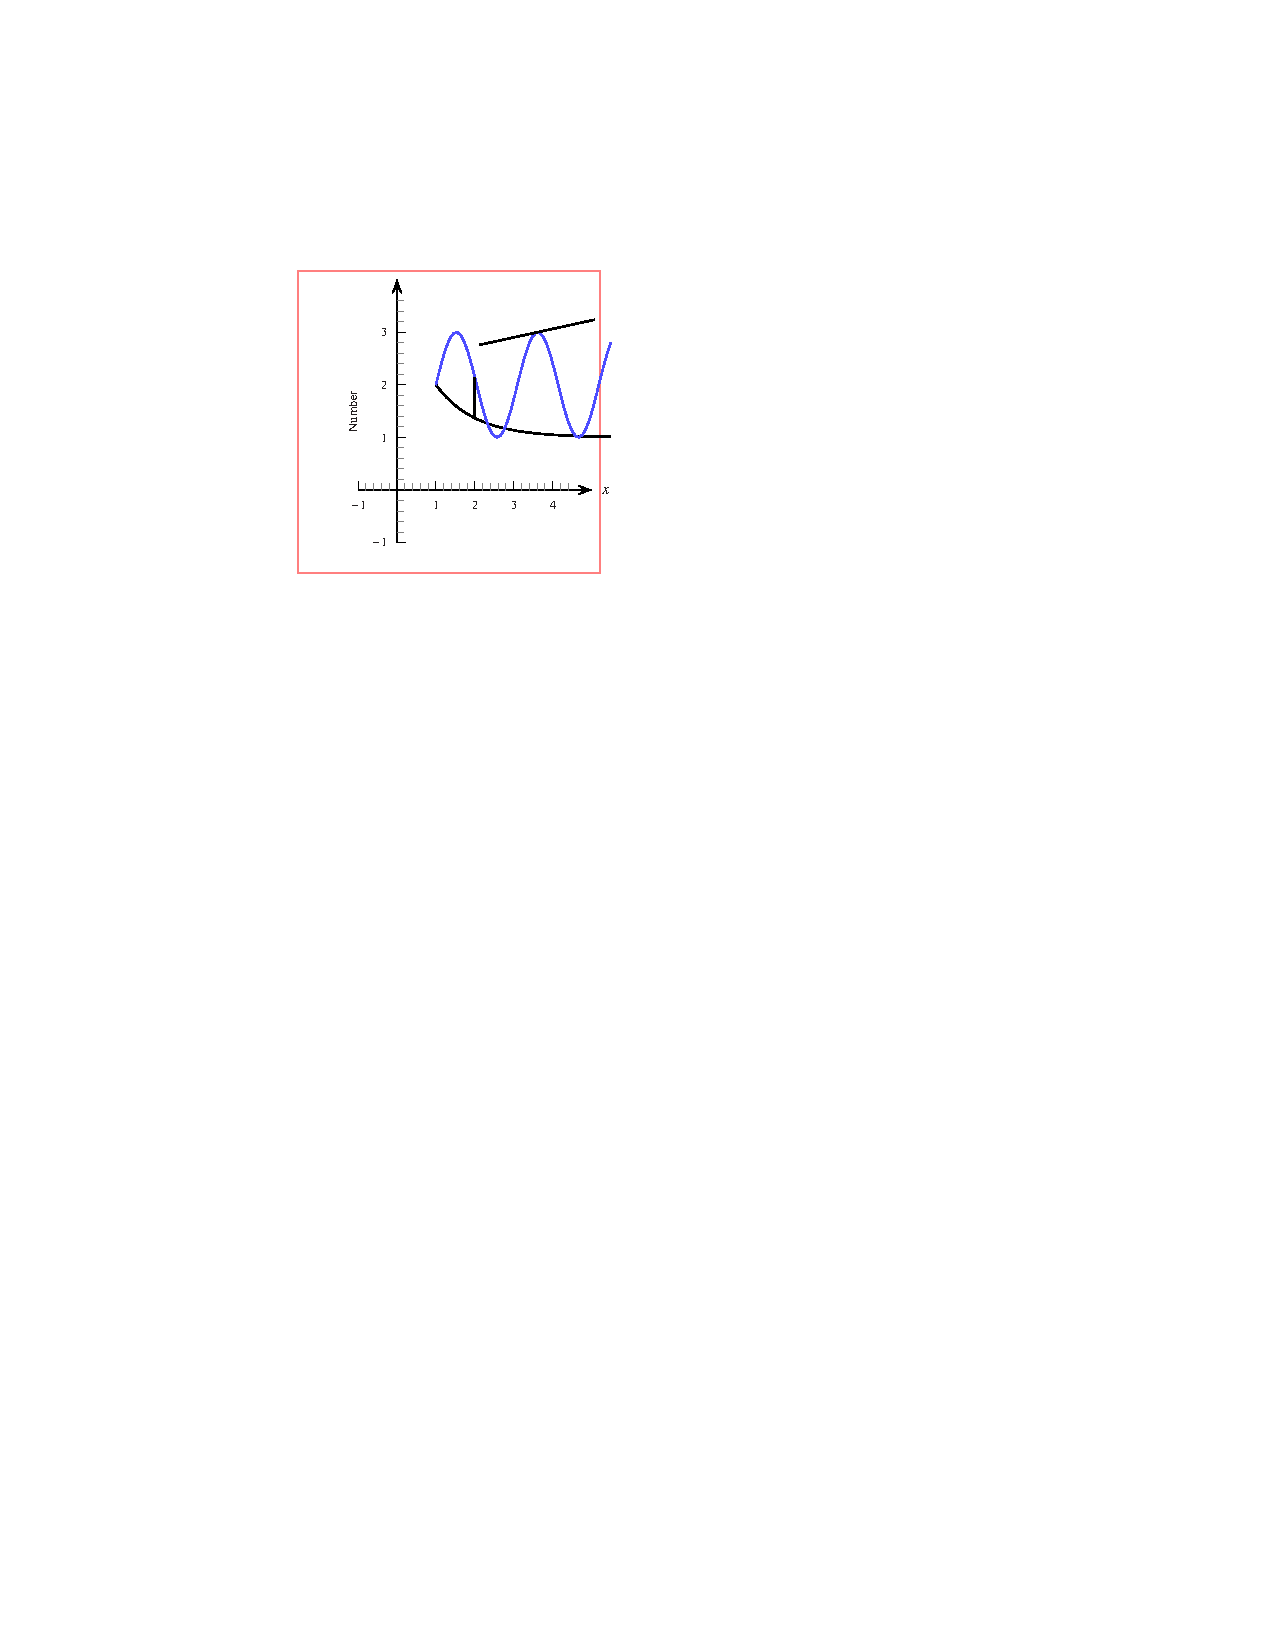
\includegraphics[viewport=165 530 300 700,clip]{pic1}} 
\endpicture\endgroup\newpage
\end{verbatim}
(A useful variant of this technique was suggested by my colleague Gill Williamson. Suppose your starting point is a hand-sketched graph or some other mathematical illustration. Scan the sketch and create a one-page document as described above on which you will make embellishments such as labels, then save this with no grid and import that document into your final larger document. This protects you from having to make many individual changes if you change the size of your picture so that  the \verb|\put()| coordinates all have to be changed.)
\newpage
\initviewport{1}{1in}{1in}{8cm}{12cm}
\scanpage{}
%viewport=xl yl xr yr
\put(100,200){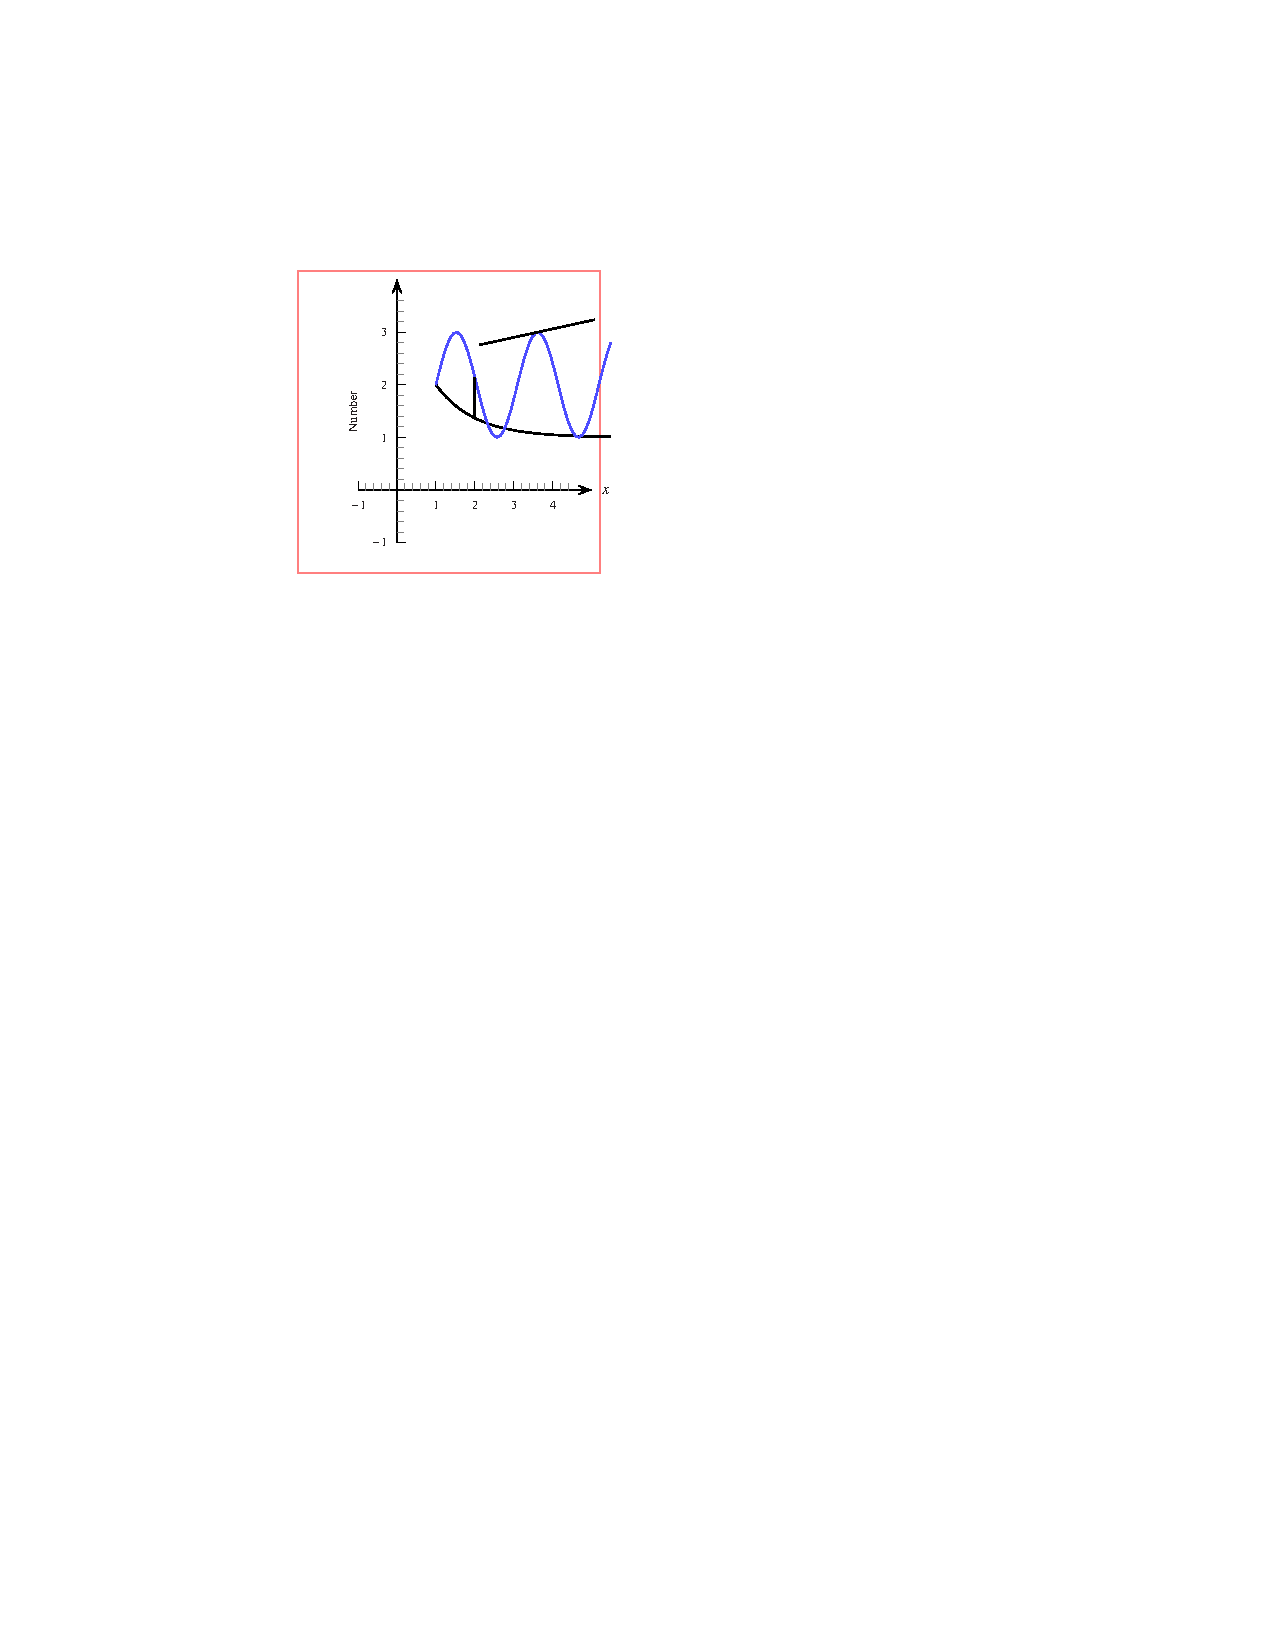
\includegraphics[viewport=165 530 300 700,clip]{pic1}} 
\endpicture\endgroup\newpage
\end{document}  